% !TEX encoding = UTF-8 Unicode

\documentclass[9pt]{amsbook}
\usepackage[b5paper,margin=1in]{geometry}
\usepackage{kerbal-book}
\usepackage{graphicx}

\usepackage{tikz}
\usepackage{pgfplots}
\usepackage{mathtools}

\usepackage{multirow}
%\usepackage[korean]{babel}


\usepackage{makecell}

\usepackage{threeparttable}
\usepackage{standalone}
\usepackage{booktabs, dcolumn}

\usepackage{subfig}
\usepackage{footnote}
\makesavenoteenv{tabular}
\makesavenoteenv{table}


%\setlength{\voffset}{- 0.3 in}
\setlength{\footskip}{40pt}

\setlength{\parindent}{1.2em}
\setlength{\parskip}{0.8em}
\renewcommand{\baselinestretch}{1.5}

\newcommand{\dia}{$\diamondsuit$}

\newcommand{\ttuna}{\textsuperscript{$\dagger$}} % Table Note 1
\newcommand{\ttsecu}{\textsuperscript{$\ddagger$}} % Table Note 2


\usepackage{fancyhdr}
\usepackage{pdflscape}
\usepackage{longtable}

\title{kerbal-book}
\author{Alberto Liberio Humaniense Disciplino}
\date{March 2016}

\begin{document}

\maketitle
\sf
%\frontmatter
\chapter*{Kerbal Space Program이란?}
\tableofcontents
%\mainmatter
\part{시작하기}
\chapter{궤도에 올리기}
\section{운동에너지 얻기}
\paragraph{일의 공식}
일의 공식은 $W=\vec{F} \cdot \vec{v} = F v \cos\theta$이다. 
즉, 힘의 방향이 운동방향과 나란할 수록 얻는 운동에너지가 많아진다. 
따라서 로켓을 발사할 때는 속도 방향과 최대한 가까운 방향으로 가속해주는것이 가속효율에 도움이 된다.
단, 에너지는 기준계에 따라 달라지므로 어떤 기준계에서 생각하는지가 중요하다. 
어떤 행성 주위에 궤도를 형성하고 싶다면 그 행성을 기준으로 한 좌표계에서 생각해야 한다. 
KSP에서는 어떤 행성이나 위성 가까이에 있으면 그 별을 중심으로 하는 관성계를 기준으로 삼고 있다 (comoving inertial frame). 
태양이나 모행성에 의한 기조력은 생각하지 않고 있으므로 훨씬 간단하게 계산할 수 있지만, 또한 나름 실제와 비슷한 현상을 이와 같은 저차근사에서도 볼 수 있다. 
주의해야 할 점은 기준계를 행성표면을 따라 자전하는 좌표계로 잡게 되면 비관성계의 역학을 적용해야 하므로 뉴턴역학을 적용할 수 없다는 점이다. 
따라서, 공기역학을 다루지 않고 순전히 탄도학만 생각할 때는 관성계를 항상 기준으로 해야함을 잊지 않아야 한다.

\paragraph{Gravity turn}
처음 로켓을 발사할 때는 수직으로 발사하게 된다. 하지만 행성 주변으로 원운동 (혹은 타원운동)을 하게 하기 위해서는 지면과 수평방향의 속도를 주는 것이 중요하다. 
이 때, 로켓의 방향을 수직에서 수평으로 눕혀주는 속도가, 앞에서 말한 바와 같이 에너지 효율에도 중요하고, 로켓의 공기역학적 안정성에도 중요하다. 
이러한 각도변화는 인위적으로 조정해야 하지만 (pitch manuever) 어느 정도 중력에 의해 자연적으로 일어난다 (gravity turn).
여기서는 이러한 turn이 자동적으로 이루어지는 이유와 정도에 대해서 우선 설명하고, 그 다음 이러한 turn을 얼마나 조정해야 하는지 설명하도록 할 것이다.


%pitch manuever
%\section{공기저항}

단, 대기밀도가 높은 곳에서는\footnote{고도 40km이하, 정확한 데이터가 있으면 추가바람.}

\section{공기역학 및 안정성}


%MaxQ

\subsection{Over-compensating}
\section{재진입시 주의사항}
\subsection{방열판 (Heat Shield)}
우주선의 대기속을 빠른 속도로 지나가게 되면, 우주선 앞쪽에는 다른 곳으로 가지 못하고 우주선 앞부분에 공기입자들이 쌓이게 되고, 반대로 우주선 뒷부분은 주변보다 공기가 적게 된다. 또한, 이런 과정은 순식간에 일어나므로, 단열압축, 단열팽창에 해당된다. 따라서, 우주선 앞부분의 고기압은 '공기저항'을 만들어 우주선을 감속시켜 주기도 하지만, 단열압축으로 인한 막대한 열로 우주선을 위협하기도 한다.

특히, 고고도에서 수직낙하할 경우에는, 
일반적인 우주여행에서 있을 수 없는 정도의 극한적인 공기저항을 받게 되므로 우주선이 타버리게 된다. 
처음 KSP를 시작하고 로켓제작에 아직 적응되지 않았을 때, 
로켓이 내는 에너지가 충분한지 알기 위해 수직발사 하는 경우가 
있을 수 있는데,\footnote{공기저항을 무시하면 대략 고도 740km이상 올라갈 수 있으면 저궤도를 구성할 수 있다.}
일반적인 경우처럼 수평과 가깝게 대기권에 들어오지 않고 거의 수직으로 대기에 재진입하게 되므로,
충분히 감속되기 전에 밀도가 높은 대기를 만나게 되어 아주 높은 열을 
내게 된다.\footnote{사실 가장 낮은 궤도에서 재진입하는 경우 v1.03에서는 방열판 없이도 살아남을 수 있지만, 
이것이 거의 유일한 상황이다.} 
따라서, 처음 로켓을 만드는 분들도 Command module밑에 방열판을 붙이는 것을 잊지 말아야 한다.

\paragraph{단열압축}
일반적인 공기저항 공식은 다음과 같다.
\begin{align}
\Delta P = \frac{C}{2} \rho v^2 = \frac{C}{2} v^2\frac{m P}{kT}
\end{align}
여기서 $m$은 공기의 평균 분자 하나당 질량이다.

여기서 이원자분자기체의 단열압축 공식은 $P^{-2}T^7=const$이므로, $\Delta P$를 $\int dP$로 해석해서 연속체공식을 구하면 다음과 같다.
\begin{align}
	\frac{7}{2}\Delta(P^{2/7}) = \frac{mP_0^{2/7}}{kT_0} \frac{Cv^2}{2}
\end{align}
제대로된 우주선의 재진입이라면 대기의 상층부에서 대부분의 감속이 일어나므로, 저압력점이 고압력점에 비해 배경 압력과 차이가 많이 나지 않는다고 가정하면, 물체 앞쪽의 단열압축에 의한 온도상승은 다음과 같다.
\begin{align}
T-T_0 = \frac{mCv^2}{7k}
\end{align}
KSP에서는 재진입 상황에서 2700K(2300m/s)에서 14000K(53000m/s)까지 도달할 수 있다. 우주선의 내열 온도는 보통 1000도 정도이므로 반드시 방열판을 설치해야만 우주선을 보호할수 있다.

\paragraph{카탈로그}
\begin{tabular}{|r|r|r|r|r|}
\hline
크기&질량& Max. Temperature& 내구 충돌속도& Ablator
\\\hline
1.25\,m&0.3\,t& 3300\,K&9\,m/s&200
\\2.50\,m&1.3\,t&3300\,K&9\,m/s&800
\\3.75\,m&2.8\,t&3300\,K&9\,m/s&1800
\\10.00\,m&1.5\,t&3500\,K&9\,m/s&-
\end{tabular}

여기서 Max. Temperature의 의마를 혼동해서는 안된다. 저자의 추측이지만 (검증바람) Max. Temp.에 도달하고 나서 부품이 바로 부서지는 것이 아니라, 그 온도 이상부터는 부품의 내구도를 소비하게 되고, 내구도가 떨어지면 파괴된다. (그렇지 않다면 내구도가 닳기 시작하는 온도가 따로 써져 있어야 할텐데 그런 온도는 없다.) 따라서, 방열판도 Max. Temp.가 되서부터야 Ablator를 소비할 것이다.

Ablator란 방열판의 양으로서, 방열판은 고온에서 기화되면서 열을 흡수하게 된다. Max. Temp. 이상이 되면 방열판의 Ablator가 소비되기 시작하고, 이것이 떨어지면 방열판은 더 이상 기능할 수 없게 된다.
\paragraph{매뉴버}

\begin{figure}
\caption{}
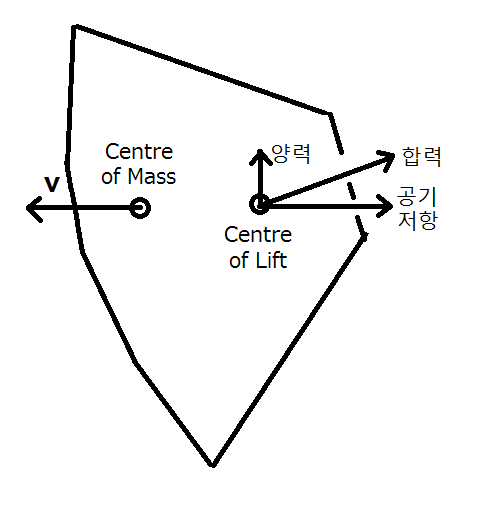
\includegraphics[width=0.3\textwidth]{lift.png}
\end{figure}

\subsection{낙하산 (Parashute)}
\paragraph{자유낙하}

\paragraph{낙하산의 종류와 전개 조건}
\begin{tabular}{|ll|r|r|r|r|}
\caption{(From Wiki and Game)}
&이름&크기&면적&작동최대속도&작동최저기압
\\
\end{tabular}

0.002atm 0.004atm

\paragraph{legacy: v1.0 미만에서의 자유낙하}
가장 일반적으로 쓰이는 공기저항 공식은 면적에 비례하지만, 
베타버전에서는 물리모델을 더 단순화시키기 위해 공기저항은 물체의 질량과 공기저항계수의 곱에 비례했다.
대부분의 물체의 저항계수는 1이었으므로,
대부분의 물체에 적용되는 종단속도가 존재했다.
또한, 대기모델도 압력이 지수함수로 감소하는 단순한 모델을 가지고 있었으므로,
공기저항에 의한 궤도변화도 계산하기 쉬웠다.

당시 공기저항 모델과 저자가 측정한 공기저항계수는 (아마 exact) 다음과 같았다.
\begin{align}
F_{drag}&=-(9.784\times 10^{-4}\, \mathrm{atm}^{-1}\mathrm{m}^{-1})\, p\, v^2
\\p&=(1 atm)\,e^{-h/h_0}
\\1\,\mathrm{atm} &:= 101325\,\mathrm{Pa}
\\h_0&:= 5\,600\,\mathrm{m}
\end{align}
\begin{center}
\begin{threeparttable}
	\caption{베타 버전에서의 고도에 따른 종단속도. 이 때는 global한 종단속도가 존재했다. (From Wiki and 직접계산)}
		\begin{tabular}{|r|r|r|r|r|}
			\cline{1-2}\cline{4-5}
			height& term. speed&&height& term. speed
			\\\cline{1-2}\cline{4-5}
			1\,000\,m&110.5\,m/s$^\flat$ && 20\,000\,m&716.0\,m/s
			\\\cline{1-2}\cline{4-5}
			2\,000\,m&121.9\,m/s && 23\,000\,{m}&961.9\,m/s
			\\\cline{1-2}\cline{4-5}
			3\,000\,m&134.5\,m/s && 25\,000\,{m}&1171.1\,m/s
			\\\cline{1-2}\cline{4-5}
			4\,000\,m&148.4\,m/s && 30\,000\,{m}&1915.4\,m/s
			\\\cline{1-2}\cline{4-5}
			5\,000\,m&163.7\,m/s && 32\,000\,{m}&2332.1\,m/s
			\\\cline{1-2}\cline{4-5}
			6\,000\,{m}&180.6\,m/s && 32\,136\,{m}&Max enter periapsis\ttuna
			\\\cline{1-2}\cline{4-5}
			7\,000\,{m}&199.3\,m/s && 35\,000\,{m}&3133.2\,m/s
			\\\cline{1-2}\cline{4-5}
			8\,000\,{m}&219.9\,m/s && 40\,000\,{m}&5125.4\,m/s
			\\\cline{1-2}\cline{4-5}
			9\,000\,{m}&242.6\,m/s && 45\,000\,{m}&8384.8\,m/s
			\\\cline{1-2}\cline{4-5}
			10\,000\,{m}&267.7\,m/s && 50\,000\,{m}&13717.9\,m/s
			\\\cline{1-2}\cline{4-5}
			12\,500\,{m}&342.4\,m/s && 55\,000\,{m}&22444.3\,m/s
			\\\cline{1-2}\cline{4-5}
			15\,000\,{m}&437.8\,m/s && 60\,000\,{m}&36724.0\,m/s
			\\\cline{1-2}\cline{4-5}
			\multicolumn{3}{r|}{}&69\,077\,{m}&End of atmosphere\ttsecu
			\\\cline{4-5}
		\end{tabular}
	\begin{tablenotes}
		\item [$\dagger$] 물체가 멀리서부터 대기로 진입할 때 이 고도보다 낮은 고도가 근지점인 궤도로 들어오면
						 공기저항이 충분하여 Kerbin에 무사히 착륙할 수 있다.
						 현재 버전에서는 이 고도보다 낮아진 듯 하다. (우주선 모양에 따라 다름)
		\item[$\ddagger$] $10^{-6}\,\mathrm{atm}$이 되는 고도이다. 여기서부터는 대기가 없는 것으로 가정하고 공기역학은 계산되지 않는다. 정식 버전의 대기모델은 훨씬 복잡하고 (지구처럼 층 구조가 있다) 대기가 끝나는 것으로 가정하는 고도는 70\,000\,m\,로 딱 떨어지는 숫자로 맞추어 놓았다. 다른 행성의 경우에는 지표면 기압의 $10^{-6}$가 대기 한계였다. 
		\item[$\flat$] 지표면 가까운 곳에서의 (10km 이하) 종단속도는 Command Module의 경우 (보통 Kerbin 귀환시) 이 속도보다는 정식버전에서 낮아져있다.
	\end{tablenotes}
\end{threeparttable}
\end{center}

\chapter{다단 로켓과 $\Delta v$}
\section{연료}

\begin{align}
    \Delta v =I_{sp}\, g_0\log\frac{M+m}{M}
\end{align}

\begin{align}
    \Delta v = I_{sp}\, g_0\log\frac{M+(1+\alpha) m}{M+\alpha m}
\end{align}
\begin{align}
    \Delta v \rightarrow I_{sp}\, g_0\log(1+\alpha^{-1})
\end{align}

is independent of thrust force but only depend on isp and etc

Let's assume $I_{sp} =320 s$ and 

Estimated Engine Mass / Fuel Mass = 1/6

Estimated Fuel Tank Mass / Fuel Mass = 1/8

$\Delta v = 4669.78 m/s$

실제로는 1단의 경우 공기저항으로 인해 연료를 많이 실을 수록 오히려 얻을 수 있는 운동에너지가 줄어드는 결과를 보이기도 한다. 따라서 많은 양의 화물(Load)을 쏘아 올리기 위해서는 `다단 로켓 (multi-stage rocket)'과 `아스파라거스 로켓 (asparagus-staging rocket)'이 필요하다.


%{\fontfamily{omyglm}가나다}
%{\fontfamily{omyglm}\selectfont가나다}
%{\fontfamily{unbtbco04}\selectfont가나다}
\section{다단 로켓 (Linear Staging)}
a


\section{아스파라거스 (Asparagus Staging)}

\section{$I_{sp}$}
\begin{align}
I_{sp} = \frac{F}{\dot{m}g_0}
\end{align}


\chapter{궤도운동}
\section{용어설명 및 주의사항}
*근일점은 꼭 태양과 지구사이만의 의미가 아니고 일반적으로 사용할것임
\section{원궤도}
\section{타원궤도}
별 (start) 우주선 (projectile) 위치에너지 (potential energy)
\begin{align}
&r^2 \dot{\theta} = l
\\&\ddot{r}-\frac{l^2}{r^3}+\frac{GM}{r^2} = 0
\end{align}
\begin{align}
	-l^2r^{-2}\frac{d^2r^{-1}}{d\theta^2}-l^2r^{-3}+GMr^{-2} = 0
\end{align}
\begin{align}
	\frac{d^2r^{-1}}{d\theta^2}+r^{-1}-GMl^{-2} = 0
\end{align}

이러한 우주선(projectile)의 운동방정식의 해는 다음과 같다.
\begin{align}
	r^{-1} = \frac{GM}{l^2} + \sqrt{\frac{2\epsilon}{l^2}+\left(\frac{GM}{l^2}\right)^2}\cos(\theta+\theta_0)
\end{align}
여기서 $\epsilon$은 우주선(projectile)의 질량당 총 에너지이다. 이러한 식은 이차곡선(원, 타원, 포물선, 쌍곡선)을 나타내는 표현이다. 따라서 이는 역제곱힘에서의 궤도가 이차곡선이 된다는 증명이다.
이 식을 $l$과 $\epsilon$이 아닌 $l$과 근일점($r_p$)의 함수로 나타내면 다음과 같이 나타낼 수도 있다.
\begin{align}
	r^{-1} = \frac{r_p^{-1}}{2}\cdot\frac{1}{1+\epsilon (GM)^{-1}r_p} +\frac{r_p^{-1}}{2}\cdot\frac{1+2\epsilon (GM)^{-1}r_p}{1+\epsilon (GM)^{-1}r_p}\cos(\theta+\theta_0)
\end{align}
$r$이 무한대로 가지 않고 유한한 영역에서 진동하고 있으면 원이나 타원, 즉 구속궤도(bound orbit)이 되고, $r$이 무한대, 즉 $r^{-1}=0$인 지점이 있으면 비구속궤도(unbounded orbit)가 될 것이다.

\section{쌍곡선궤도 - 탄성충돌}
\section{슬링샷}

\begin{align}
	\Delta \theta = \pi + 2\sin^{-1}\frac{1}{{1+2\epsilon (GM)^{-1}r_p}}
\end{align}
\textbf{\textsf{\large 특akak}}\;\; aaa

\paragraph{충돌각 최대값}
\begin{center}
\begin{threeparttable}
\begin{tabular}{|c|c|c|c|c|c|c|}
모행성&Entry Speed$^\dagger$& 위성& Radius& Lowest Safe Altitude\footnote{행성의 가장 높은 지점의 고도와 대기의 두께 중 큰 것}&원지점 공전속도 &최대 슬링샷 각도
\\\hline
Eve&Gilly
\\\hline
Kerbin&Mun
\\&Minmus
\\\hline
Duna&Ike
\\\hline
Jool&Laythe
\\&Vall
\\&Tylo
\\&Bop
\\&Pol
\end{tabular}
\begin{tablenotes}
\item[$\dagger$] 행성들의 궤도를 같은 궤도면상 원궤도로 가정하면 모행성계로 Hoffman Transfer 할 때 행성계 기준에서의 속도
\end{tablenotes}
\end{threeparttable}
\end{center}
모행성 이심률 0.1이하
\paragraph{특정 기준계에 대한 슬링샷 결과}
어떤 기준계에 대해서 우주선의 입사 속도가 $\vec{v}_s(t=-\infty)$, 천체의 속도가 상수 $\vec{v}_c$라고 한다면, 위와 같은 계산결과에 따라 우주선의 최종 속도가 어떻게 되는지 계산해보자.

우선 천체계에서 우주선의 속도는 $\vec{v}_s(t=-\infty)-\vec{v}_c$가 될 것이다.

예) 달을 이용한 가속
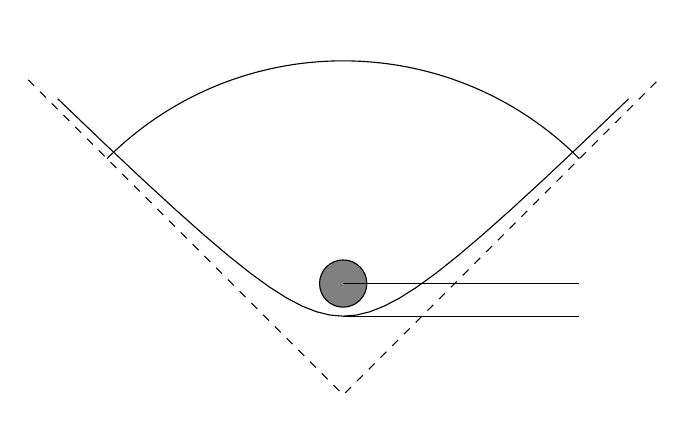
\begin{tikzpicture}
\draw[fill=gray] (0,{sqrt(2)}) circle (.3);
\draw [dashed] (-4,4)--(0,0)--(4,4);
\draw plot[domain=-2:2, thick] ({sinh(\x)},{cosh(\x)});
\draw (0,{sqrt(2)})--(3,{sqrt(2)});
\draw (0,1)--(3,1);
\draw[thin] (-3,3) arc (135:45:{3*sqrt(2)});
\end{tikzpicture}

진입속도 $v$, 근접거리 $r$.

\chapter{달 미션}

\part{매뉴버}
\part{미세조정 (Fine-tuning)}
\part{행성간 비행}
\chapter{시간계획 정하기}
\chapter{포획 (Capturing)}
행성계 외부에서 진입하는 물체는 탈출속도를 넘어서므로\footnote{정확히는 `행성계 관점에서 보았을 때 양(陽)의 에너지를 갖으므로'라고 하는 것이 옳을 것이다. `탈출속도'라는 개념은 보통 원궤도를 그리던 물체에 얼마만큼의 $\Delta v$가 주어져야 탈출할 수 있는지에 대한 얘기이다.} 힘이 작용하지 않으면 쌍곡선 궤도를 그리며 다시 행성계 밖으로 탈출하게 될 것이다.
안정적인 미션 수행을 위해서 행성간 미션에서는 도착지에서 충분히 감속하여 구속궤도를 만들 수 있는 기술이 필요하다. 이를 `포획'이라고 부르도록 하겠다. 포획이 이루어지지 않는다면 행성의 인공위성 궤도에 진입하는 미션을 수행할 수 없으며, 착륙 미션에 경우 한번만에 성공해야 하는 부담을 안게 된다.\footnote{비구속궤도(쌍곡선궤도)로부터 대기권으로 진입할 때, 높은 진입속력으로 인해 높은 열이 발생하게 되어 우주선이 소실될 위험성이 커지게 되며, 또한 다시 튕겨나가지 않고 충분히 감속할 수 있는 가능성도 줄어들게 된다.}

엔진을 이용한 능동적인 감속은 설명이 필요없으므로 여기서는 동력을 사용하지 않고 포획당하는 방법에 대해서 설명하고자 한다. 두가지 방법을 생각할 수 있을텐데, 행성의 대기를 이용한 방법과 행성의 위성을 이용한 방법이 있을 것이다. 각각의 방법에 대해서 설명하고자 한다.
\section{대기를 이용한 포획 (Atmospheric Capture)}
\section{위성을 이용한 포획 (Sling-shot Capture)}
다음은 위성을 이용한 슬링샷으로 행성계에서의 속도를 줄일 수 있는지 검토해 보도록 하자. 위성과 조우시 위성의 속도가 우주선의 반대방향이라면 위성의 운동량을 받아 감속할 수 있으리라고 예상할 수 있을 것이다. 하지만 행성간 여행에서 그렇게 정확한 타이밍을 맞출 수 있으리라고 기대하기는 어렵다. 이번 section에서는 행성계 진입후 주어진 상황에서 감속할 수 있는지에 대해 알아볼 것이다. 다음 section에서는 진입 타이밍을 조정하는 법에 대해 논의해 보겠다.

우선 행성과 위성은 충분히 멀리 떨어져 있어서 조우(encounter)를 탄성충돌로 근사할 수 있다고 가정할 것이다. 사실 KSP는 각 천체의 '영향권'내에서 1체문제로 환원함으로서 이러한 가정을 충실히 따르고 있다.
\section{포획을 위한 궤도조정 (Fine-tuning with Sling-shot Capture)}

\chapter{사례들}
\section{Juno's Maneuver}
\begin{enumerate}
\item 지구계를 탈출한다.
\item 약 2배의 공전궤도를 만들어 다시 지구와 만날 수 있게 한다.
\item 원일점에서 근일점을 낮게 하는 매뉴버를 실시하여 다음 매뉴버에서의 에너지 효율을 높인다.
\item 지구를 이용한 슬링샷 효과를 포함하여 목성과의 접점을 만든다.
\item 목성근체에서 목성과 비슷한 속도로 가속하여 목성궤도로 들어간다.
\end{enumerate}
\part{그 외 다루어지지 않은 것들}
\chapter{Aviation}
이번 chapter에서는 비행기로 비행시에 유용하게 쓸 수 있는 도표를 소개하고자 한다.

비행기의 비행속도 측정시에 IAS(Indicated Airspeed)라는 단위를 쓰게 된다. 
이는 비행기 바깥에 붙어있는 압력계를 이용하여 공기밀도를 표준밀도로 가정하고 공기의 유속을 추정한 결과로서, 베르누이 법칙($\rho v^2 + P = const$)을 고려해보자면 계기에 의해 측정되는 수치는 같은 유속일때 유체의 밀도의 (-1/2)승에 비레하게 될 것이다. (반대로 True Airspeed를 구하기 위해서는 측정된 압력차에 공기밀도의 제곱근을 곱하면 될 것이다.)

한편, 공기저항 또는 양력(lift)은 보통 저속에서 면적과 공기밀도에 비례하고 속도의 제곱에 비례한다는 공식을 쓴다. ($\sim \rho v^2 A$)
두 공식이 $\rho v^2$에 비례한다는 점에서 같으므로 양력은 IAS에만 의존하게 된다고 할 수 있다. (물론 고속에서 양력 공식이 변한다면 이 또한 달라질 것이다.)

저자가 실제로 게임 상에서 실험해본 바로는, 실제 지구처럼 시각에 따라, 태양복사에 따라 대기의 온도가 변하는 듯하지만, 위키에 제시된 Kerbin 표준 기온 도표에 따라 계산하도록 하겠다. \footnote{\url{http://wiki.kerbalspaceprogram.com/wiki/Kerbin}}

\paragraph{종단속도}
흡기하는 제트엔진의 추력은 어림잡아 공기밀도에 비례한다고 예상할 수 있다. (실제 게임에서는 어떤 모델을 쓰는지 모르겠음. 추가바람. 특히, 램제트 같은 고속에 특화된 엔진 및 흡기구의 경우 많이 달라질 수 있음.) 또한, 공기저항도 어림잡아 공기밀도에 비례하므로, 비행기의 종단속도는 고도에 따라 변하지 않는다고 예상할 수 있다.
\begin{figure}
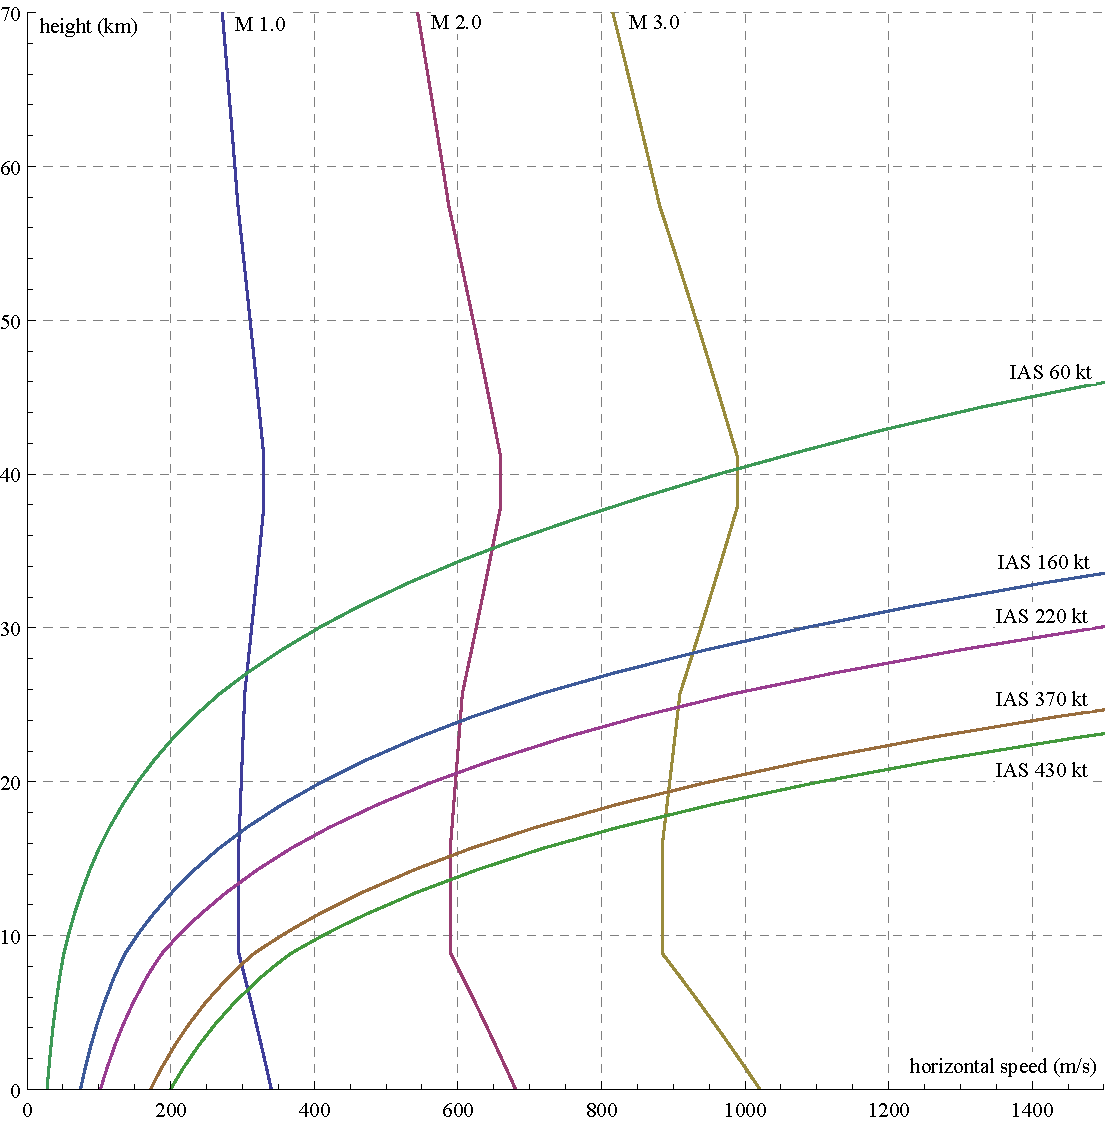
\includegraphics[width=\textwidth]{ias.pdf}
\caption{test 참고로 대략적으로 IAS 60\,kt\,는 경비행기의 이착륙속도이고 IAS 160\,kt, 220\,kt는 각각 B747과 Concorde의 이착륙속도이다. IAS 370\,kt와 430\,kt는 747과 Concorde의 순항속도이다. 실제 지구에서 Concorde는 55,000\,ft에서 M\,2.0으로 항행하였다.}
\end{figure}

경험상 흡기엔진으로 구동하는 비행기가 항속 가능한 최대고도 및 속도는 23000\,m 및 1200m/s 정도였다. (정확한 자료 추가바람. 하지만 비행기의 모델에 따라 달라지므로 정말 '극한값'을 구할 수 있을지는 미지수.) 
또한, 흡기 자체는 26000\,m 까지 가능하였다. (속도에 따라 달라질 수 있다.)

\chapter{3체 문제 (Three Body Problem)}
\section{KSP의 간략화}
\section{근일점 변화}
\begin{align}
	\frac{d^2r^{-1}}{d\theta^2}+r^{-1}-GMl^{-2}-l^{-2}r^2V'(r) = 0
\end{align}
\begin{align}
	\frac{d^2r^{-1}}{d\theta^2}+r^{-1}-GMl^{-2}+2 l^{-2}r^3 \left(\frac{|\alpha_-| -|\alpha_+|}{2}+\frac{|\alpha_-| +|\alpha_+|}{2}\cos(\theta-\omega t)\right)= 0
\end{align}


\section{세차운동}
*로켓발사로 인한 변화
\\*애초에 축은 0도로 고정
\chapter{상대론적 문제}
\section{특수상대론: 로렌츠변환}
\section{특수상대론: 적색/청색편이}
\section{일반상대론적 효과 및 천체모델의 근사성}

\part{데이터 및 프로토콜}
\chapter{게임 데이터}
이 챕터의 내용은 주로 게임 내부 데이터 및 물리법칙에 대한 것이며, 
따라서 저작권은 게임제작사에 있으며, 인용하고 있는 제3자의 저작권은 없는 것으로 해석한다. (독창성 결여)
%데이터는 게임 플레이 중 직접 확인할 수 있는 부분이며, 상이한 점을 발견하면 갱신 부탁드립니다.
데이터는 게임 플레이 중 직접 확인할 수 있는 부분이며, 상이한 점이 있다면 github에서 직접 갱신할 수 있다.

인용처는 다음과 같다.
\begin{itemize}
\item 게임에서 직접 확인한 정보 인용
\item 참고: ``Kerbal System Celestial Body Parameters in v0.18.2'' \url{https://docs.google.com/spreadsheets/d/1HwrFq6r2Wfzvghq8VYMNx0F2rG6nYMAEl_cyLj2EXjA/edit#gid=0}\footnote{I obtained this sheet from some forum but I forgot where it was. Sorry for that.}
\item 참고: \url{http://wiki.kerbalspaceprogram.com/}
\end{itemize}

\section{행성 데이터}
KSP에서 행성과 위성의 운동은 물리법칙의 시뮬레이션에 의한 것이 아니라 고정된 주기를 가진 고정된 운동궤도에 따른 것입니다. 공전주기와 공전궤도는 항성 또는 모행성이 아주 무겁다고 생각하고 만들어진 1체문제의 해이며, 모행성의 위성에 의한 흔들림 등은 전혀 고려되어 있지 않습니다.
\begin{landscape}
%\begin{center}
%\resizebox{\textheight}{!}{
\begin{adjustbox}{width=15.5 cm}%\textheight}
\begin{threeparttable}
\caption{(From Wiki and Forum)}
\begin{longtable}{|l|r|r|r|r|r|r|r|r|r|r|r|r|r|}
\hline
이름&$GM$\ttuna ($\mathrm{m}^3/\mathrm{s}^{2}$) &반지름&원일점$^\ast$&근일점$^\ast$%&공전주기\ttsecu
&자전주기$^\star$ &LAN$^\sharp$&INC$^\natural$&LPE$^\S$&MNA$^\flat$ &대기한계& 최고지점&지표면기압
\\\hline
Sol&$1.172\,332\,8\times 10^{18}$&261\,600\,000\,m&-&-&432\,000.000\,s&-&-&-&-&600\,000\,m&-&16\,kPa
\\\hline
Moho&$1.6860938\times 10^{11}$&250\,000\,m&6\,315\,765\,980\,m&4\,210\,510\,628\,m
%&2\,215\,754.220\,s
&1\,210\,000.000\,s&70.00$^\circ$&7.000\,$^\circ$&15.0\,$^\circ$&3.140\,rad&0&6\,817\,m&0
\\
Eve&$8.1717302\times 10^{12}$&700\,000\,m&9\,931\,011\,387\,m&9\,734\,357\,701\,m
%&5\,657\,995.1\,s
&80\,500.000\,s&15.00$^\circ$&2.100\,$^\circ$&0.0$^\circ$&3.140\,rad&90\,000\,m&7540\,m&506.625\,kPa
\\
Kerbin&$3.5316000\times 10^{12}$&600\,000\,m&13\,599\,840\,256\,m&13\,599\,840\,256\,m
&21\,549.425\,s&80.00$^\circ$&0&0.0$^\circ$&3.140\,rad&70\,000\,m&6764.1\,m&101.325\,kPa
\\
Duna&$3.0136321\times 10^{11}$&320\,000\,m&21\,783\,189\,162\,m&19\,669\,121\,365\,m
&65\,517.859\,s&135.50$^\circ$&0.060\,$^\circ$&0.0$^\circ$&3.140\,rad&50\,000\,m&7\,5**\,m&6.755\,kPa
\\
Dres&$2.1484489\times 10^{10}$&138\,000\,m&46\,761\,053\,522\,m&34\,917\,642\,884\,m
&34\,800.000\,s&280.00$^\circ$&5.000\,$^\circ$&90.0$^\circ$&3.140\,rad&0&5\,7**\,m&0
\\
Jool&$2.8252800\times 10^{14}$&6\,000\,000\,m&72\,212\,238\,387\,m&65\,334\,882\,252\,m
&36\,000.000\,s&52.00$^\circ$&1.304\,$^\circ$&0.0$^\circ$&0.100\,rad&200\,000\,m&-&1519.875\,kPa
\\
Eeloo&$7.4410815\times 10^{10}$&210\,000\,m&113\,549\,713\,200\,m&66\,687\,926\,800\,m
%&156\,992\,048.4\,s
&19\,460.000\,s&50.00$^\circ$&6.150\,$^\circ$&260.0$^\circ$&3.140\,rad&0&3\,9**\,m&0
\\\hline
\end{longtable}
\begin{tablenotes}
\item[$\dagger$]질량$\times$뉴턴중력상수. Standard gravitational parameter. KSP에서는 질량이 아니라 이 값이 exact하게 정의되어 있다.
%\item[$\ddagger$] 원일점과 근일점의 종속변수이나, 컴퓨터의 계산오차가 있으므로 게임 내부적으로 상수일 것으로 생각된다.
\item[$\star$] 1항성일. 절대계 기준으로, 1태양일과는 다르다.
\item[$\sharp$] Longitude of the Ascending Node
\item[$\natural$] Orbital Inclination
\item[$\S$] Argument of Periapsis
\item[$\flat$] Mean Anomaly at Epoch UT=0
\item[$\ast$] 태양 중심으로부터의 거리 (radius). Height(태양 표면으로부터의 거리)가 아님.
\end{tablenotes}
\end{threeparttable}
%}
\end{adjustbox}
%\end{center}
\end{landscape}

\paragraph{1 Solar Day}
Different than mean solar day, a solar day varies depending on the position on the solar orbit.
There are mainly two reasons of the variation of the solar day:
\begin{itemize}
\item eccentricity of the orbit, 
\item and axial tilt or obliquity, angle between equatorial plane and orbital plane.
\end{itemize}

Under these assumptions:
\begin{itemize}
\item the Sun is much more massive than a planet so that the orbit is perfectly ellipse,
\item and a day is much shorter than an year,
\end{itemize}
we can obtain the length of a solar day depending on the position.

First, let us obtain the angular velocity on certain position using Keplar's second law.
The total area enclosed by the elliptic orbit on the orbital plane is $\sqrt{r_p r_a}\frac{r_p+r_a}{2}\pi$ where $r_a$ is the apoapsis, and $r_p$ is the periapsis radius. Thus, the areal velocity is constantly $\sqrt{r_p r_a}\frac{r_p+r_a}{2}\frac{\pi}{T}$ where $T$ is the orbital period. In conclusion, the equation to obtain the relation between solar distance $r$ and angular velocity $\omega$ is:
\begin{align}
\frac{r^2 \omega}{2} = \sqrt{r_p r_a}\frac{r_p+r_a}{2}\frac{\pi}{T}
\\\nonumber\Rightarrow \omega = \sqrt{r_p r_a}\frac{r_p+r_a}{2r^2}\frac{2\pi}{T}.
\end{align}

%두가지 요인: 공전궤도의 이심률과 자전축과 공전평면과의 각도.
%넓이:sqrt{r_p r_a}*{r_p+r_a}/2*pi
%r cross v /2 = 넓이/주기
%omega= sqrt{r_p r_a}*{r_p+r_a}*pi/r^2/주기
%omega= sqrt{r_p r_a}*{r_p+r_a}/(2r^2)* 평균각속도 (공전평면상)

%-> 자전축을 수직으로 세우면?

\section{위성 데이터}

\begin{tabular}{|c|c|c|c|c|c|c|c|c|c|c|}
%\hline
모행성&위성 이름& $GM$& 자전주기\footnote{1항성일}& 공전주기\footnote{1항성월}& 원지점&근지점&Sphere of influence&위성 반지름& 대기한계고도 & 지형 최대고도
\\
\multirow{2}{*}{Kerbin}& Mun
\\&Minmus
\end{tabular}
\section{엔진 데이터}

200 FuelUnit = 1t. (oxygen and liquid)
\\10000 FuelUnit = 1t. (Xenon)
density: expected around $1t/m^3$ (liquid)
, 1.05949191932 $m^3$ = 1t.
\\density:
0.657420 $m^3$, 0.525t xenon. (xenon)
0.0406->0.0371$m^3$,0.04t
Globally, total fuel mass : tank mass = 8:1. (round bare tank. extra structure may weigh more.)
Globally(xenon), total fuel mass : tank mass = 14:11. (round bare tank. extra structure may weigh more.)
\begin{threeparttable}
\begin{tabular}[t]{|c|c|c|c|c|c|}
\hline
&Liquid/Oxydizer& Solid& RCS& Xenon& Ore
\\\hline
Density ($t/m^3$)\textsuperscript{*}&$\sim$1&
$\sim$1&0.5$\sim$4\textsuperscript{!}&$\sim$1&$\sim$ 1.3
\\\hline
Density (t/FuelUnit)& 1/200 & 3/400 & 1/250 & 1/10000 & 1/100
\\\hline
\makecell{Least Mass Ratio 
\vspace{-2pt}
\\
\vspace{2pt}
of $\dfrac{\text{(Tank Structure)}}{\text{(Fuel Capacity)}}$}
&1/8&0.231$\sim$0.2439\textsuperscript{\textdagger}&>0.1333$\sim$0.1775&11/14&1/6
\\\hline
Cost per FuelUnit&0.8(Liq)/0.18(Oxy)&0.6&1.2&4&0.02
\end{tabular}
    \begin{tablenotes}
    \item[!] Smaller tank can store more densely.
    \item[*] Measured from the graphic
    \item[\textdagger]  Including engine
    \end{tablenotes}
\end{threeparttable}
\chapter{프로토콜}
본 챕터에서는 우주선끼리의 충돌을 피하기 위해 우주영역을 구분하거나, 달에 착륙할 때 안전하고도 효율적인 표준 프로토콜을 정하는 등, 우주 비행에 있어서의 여러가지 프로토콜(약속)들을 저자가 개인적으로 정하여 제안하여 보는 바이다.
혹시 미래에 멀티플레이어 기능이 들어가게 된다면 유용하게 쓸 수 있을 것이다.
\section{Kerbin 궤도 프로토콜}
\begin{align}
T = 2\pi \sqrt{\frac{a^3}{GM}}
\end{align}
\begin{threeparttable}
\caption{궤도 고도 프로토콜}
\begin{tabular}{|r|r|l|}
\hline
궤도고도 & 궤도이름& 용도
\\\hline
80\,km$\pm$5\,km&Insertion Orbit& 지표면에서부터 궤도에 처음 오른 우주선이 
\\&&들어서는 궤도
\\100\,km$\pm$5\,km&&
\\120\,km$\pm$5\,km&Space Station Orbit& 우주정거장이 들어설 궤도. 궤도 조정을 할 수 있게 
\\&&
Insertion Orbit에서 어느정도 거리를 두면서도,
\\&&
 에너지가 적게 드는 낮은 궤도를 선택해야 한다.
\\150\,km$\pm$5\,km&&
\\200\,km$\pm$5\,km&재급유 궤도& 광물 채취 왕복선이나 원정을 가는 우주선이 재급유
\\&&
 할 때 들를 수 있는 궤도. 바깥쪽에서 접근하기 
 \\&&
쉽도록 높은 고도의 궤도로 정한다.
\\2863.334\,06\,km&정지 궤도\textsuperscript{!}&
\\\hline
\end{tabular}
\begin{tablenotes}
\item[!] \url{http://wiki.kerbalspaceprogram.com/wiki/KEO}
\item[주의사항:] 궤도간 이동을 할 때는 충돌을 피하기 위해 다른 물체의 궤도면을 피해서 이동할 것. 특히 적도 궤도면을 피해 5도 정도의 각도를 주고 이동할 것.
\end{tablenotes}
\end{threeparttable}
\begin{table}
\caption{원형궤도 및 타원궤도에서의 원지점/근지점에서의 속도(m/s). 첫행의 고도에서의 속도가 표에 적혀있는 내용. 각 행의 첫 열은 궤도 반대편의 고도이다. 한쪽이 원지점이면 다른쪽이 근지점이 된다.}
\begin{tabular}{|r|r|r|r|r|r|r|}
\hline
&80\,km&100\,km&120\,km&150\,km&200\,km&2863\,km
\\\hline
80\,km&2278.93&2229.80&2182.86&2116.20&2014.09&578.54%540
\\\hline
100\,km&2295.39&2246.14&2199.07&2132.24&2029.83&585.57%574
\\\hline
120\,km&2311.26&2261.90&2214.72&2147.72&2045.03&592.46%459
\\\hline
150\,km&2334.04&2284.54&2237.21&2169.98&2066.91&602.52%520
\\\hline
200\,km&2369.52&2319.80&2272.26&2204.70&2101.07&618.62%620
\\\hline
2863\,km&2946.58&2897.20&2849.84&2782.30&2678.11&1009.81
\end{tabular}
\end{table}
\section{달 착륙}
실제 아폴로 착륙시에는 3단계의 매뉴버를 하였다고 한다. 우선 착륙선을 감속하여 목표지점보다 가까이 떨어지도록 한다(수평속도 감속). 그 다음, 떨어지는 속도를 감속하여 목포지점보다 약간 멀리 떨어지도록 감속한다(기존에 떨어지는 방향보다 수직방향의 속도를 우선 감속). 마지막으로 미세조정 및 역분사로 착륙의 마지막 단계이다. 이를 참고하여 제안해보고자 한다.


\backmatter
\backpage

\end{document}
